\chapter{A finite element method for the Landau-Lifshitz-Gilbert Equation}
\label{sec:galerk-meth-llg}

In this chapter we introduce first give a general introduction to the finite element method.
We then apply the finite element method (with the Newton-Raphson method for linearisation) to the Landau-Lifshitz-Gilbert equation with exchange and a simple magnetostatic field approximation.

\section{Introduction to the finite element method}
\label{sec:intr-finite-ele-diff}

As discussed in \autoref{sec:sd-finite-elem-meth} the finite element method (FEM) is a discretisation method which converts a differential equation into a system of algebraic equations.
It allows for more complex geometries than the finite difference method, at the cost of increased complexity.

A simple problem is used to illustrate these methods: solving the Poisson
equation in one spatial dimension.
This is relevant to 
Find\footnote{A function $g\in C^{k}(0,1)$ if $g$ and it's first $k$ derivatives are continuous on $(0,1)$.} $y(x)\in C^{2}(0,1)$ such that
\begin{equation}
  -y''=f\qquad\text{on }(0,1)
  \label{eq:poisson1}
\end{equation}
\begin{equation*}
  y(0)=y_{a},\quad y(1)=y_{b},\quad f=f(x)\in C(0,1).
\end{equation*}


\subsection{Definitions}
\label{sec:fem-definitions}

The function space $L^{2}$ is the set of all functions $f(x)$ such that $\int_{-\infty}^{\infty}\abs{f(x)}^{2} \d x$ is finite.
The span of a set of functions is the set of all possible linear combinations of the functions. 
If a set of functions $\set{\phi_i}$ is such that $V=\text{span}(\phi_i)$ then we say that $\set{\phi_i}$ spans $V$ and $\set{\phi_i}$ is a basis for the function space $V$.
If $V$ has a basis consisting of a finite number of functions then we say that $V$ is finite dimensional, otherwise $V$ is infinite dimensional.
In a FEM we are interested in approximating an infinite dimensional space (the space of solutions) by a finite dimensional space (the space of approximations).

The $n$-th Sobelov space is the space of all functions such that they and their $n$-th derivatives (in all dimensions) are in $L^2$. For example
\begin{equation}
  \label{eq:H1}
  \sob^1(\magd) = \set{ y \st y, \pd{y}{x_i} \in L^2(\magd) \; \forall x_i }
\end{equation}

\subsection{A weak formulation}
\label{Derivation-of-weighted-residuals}

The method of weighted residuals is a way to convert a differential equation
into an integral form that can be modelled computationally. As such it is the
first step in a variety of modelling methods including the finite element method
and the spectral method.

For simplicity we start, as before, with the one-dimensional Poisson equation
\eqref{eq:poisson1}, with homogeneous Dirichlet boundary conditions
(\ie $y_{a}=y_{b}=0$).

% \footnote{The functions must be Lipschitz continous (a stronger form
% of continuity than standard). Lipschitz continuity is defined as the
% following: for $X,Y$ metric spaces with metrics $d_{x}(x_{1},x_{2})$,
% $d_{y}(y_{b},y_{2})$ respectively then a function $f:X\rightarrow Y$ is
% Lipschitz continuous if and only if $\exists K\geq0$ s.t. $\forall
% x_{1},x_{2}\in X$ $d_{y}(f(x_{1}),f(x_{2}))\leq K\, d_{x}(x_{1},x_{2})$.}

The formulation used in \eqref{eq:poisson1} (called a strong formulation) is too restrictive for our purposes.
It disallows some useful approximating functions, and in higher dimensional cases restricts the geometries that can be modelled \cite{HowardElmanDavidSilvester2006}. 
However for well behaved functions the following weak formulation is equivalent: find $y\in V_{s}$ such that
\begin{equation}
  -\int_{0}^{1}y''v\, dx=\int_{0}^{1}fv\, dx \qquad \forall v\in V_{T}.
  \label{eq:26}
\end{equation}

Here $V_{T}$ is some appropriate space of test functions. The test
functions must satisfy $V_{T}\subseteq \sob^0(0,1)$, in order to ensure that the integrals in \eqref{eq:26} are well defined. 
Thus
\begin{equation}
  \label{eq:28}
  V_{T}=\set{v : [0,1] \rightarrow \real \st v \in \sob^0(0,1)}.
\end{equation}

The space $V_{s}$ is the solution space
\begin{equation}
  V_{s}=\set{ y : [0,1] \rightarrow \mathbb{R} \st y \in \sob^2(0,1),\, y(0) = y_{a},\, y(1) = y_{b}},
\end{equation}
\ie the space of functions that are sufficiently smooth for the integrals to be finite and that satisfy the boundary conditions.

To see that the weak form is equivalent to \eqref{eq:poisson1} consider the case when $f(x) - y''(x)$ is non-zero at a point $x \in [0,1]$. 
Since \eqref{eq:26} must hold for all functions we can choose a function which is non-zero at $x$ and hence the equality in \eqref{eq:26} fails.
So $f(x) - y''(x) = 0$ must hold at all points inside the domain.
We call this the method of weighted residuals because we use a weighted integral of the residual to approximate the true equation \cite[210, 214]{Zeinkiewicz1967}.

The smoothness restrictions on our weak form approximation can be further reduced using integration by parts
\begin{equation}
  \intui{qp'} = \Big[ pq \Big]_{0}^{1} - \intui{p q'},
\end{equation}
applied to the left hand side of equation~\eqref{eq:26}.
Let $p=y'$ and $q=v$, then
\begin{equation}
  -\intui{ y''v } = -\Big[ y'v \Big]_{0}^{1} + \intui{ y'v' }.
  \label{eq:29}
\end{equation}

We now introduce a second constraint to the test functions: $v=0$
at the boundaries (\ie $v_a=v_b=0$), so the bracketed term in \eqref{eq:29} is
zero and we are left with
\begin{equation}
  -\intui{ y''v } = \intui{ y'v' }.
\end{equation}

Hence our problem can be reduced to the following: find 
\begin{equation}
y\in V_{S}'=\set{y \st y \in \sob^1(0,1),\, y(0) = y_a, y(1) = y_b },
\end{equation}
such that
\begin{equation}
  \intui{ y'v' } = \intui{ fv } \qquad 
  \forall v \in V'_{T} = \set{v \st v \in \sob^1(0,1),\, v_a=v_b=0}.
  \label{eq:symmetric-weak-poisson}
\end{equation}

Note that this rearrangement has removed the second derivative in $y$, hence we only require $y \in \sob^1(0,1)$ instead of $y \in \sob^2(0,1)$.
This allows a wider range of shape functions to be used but comes at the expense of requiring more smoothness in the test functions.
Also note that if $y_a = y_b = 0$ then $V_{S}'=V_{T}'$, our test and solution spaces are identical.

\subsection{A Discretisation}

Equation~\eqref{eq:symmetric-weak-poisson} is still inapplicable as a computational method since the test (and solution) space is infinite dimensional (\ie the problem is still continuous).
So for the next step we approximate $V_{T}'$ by a finite dimensional function space $V_{T}^{h}\subset V_{T}'$ such that
\begin{equation}
  V_{T}^{h}=\text{span} \set{ \tbf_{\ndi} }_{n=1}^{N}
  =  \set{v_h \st v_h = \sum_{n=0}^{N}\alpha_{\ndi} \tbf_{\ndi},\, \alpha_{\ndi} \in \real,\, v_a = v_b =0 },
  \label{eq:30}
\end{equation}
for some finite set of basis functions $\tbf_{\ndi}$.
Similarly for $V_S$
\begin{equation}
  \label{eq:34}
  V_{S}^{h}=\text{span} \set{ \sbf_{l} }_{l=1}^{N_l}
  =  \set{y_h \st y_h = \sum_{l=0}^{N_l}c_{l} \sbf_{l},\,
  c_{l} \in \real,\, y(0) = y_a,\, y(1) = y_b }.
\end{equation}

We call $\sbf_l$ the \emph{shape functions}.
Different choices of $\tbf_{\ndi}$ and $\sbf_l$ lead to different methods, the choice corresponding to the finite element method will be discussed in \autoref{sub:Actual-Finite-Elements}.
For now we convert the problem into a general discrete form.

We currently have the \emph{discrete weak formulation} of \eqref{eq:poisson1}: find $y_{h}\in V_{S}^{h}$ such that
\begin{equation}
  \intui{ y'_{h}v_{h}' } =\intui{ fv_{h} } \qquad\forall v_{h}\in V_{T}^{h}.
  \label{eq:discrete-weak-prob}
\end{equation}

Replacing $v_{h}$ from \eqref{eq:discrete-weak-prob} by $\tbf_{\ndi}$ gives
\begin{equation}
  \intui{  y'_{h} \tbf_{\ndi}'  }  = \intui{ f\tbf_{\ndi} } \qquad n=0,\ldots,N,
  \label{eq:discrete_weak_test_fns_replaced}
\end{equation}

Since $y_{h}\in V_{S}^{h}$ we can also replace $y_{h}$ by a linear combination of the spanning functions, \ie
\begin{equation}
  y_{h}=\sum_{l=0}^{N_l}c_{l}\sbf_{l},
  \label{eq:y-spans}
\end{equation}
where $c_l \in \real$ are the (unknown) coefficients.

Substituting \eqref{eq:y-spans} into equation~\eqref{eq:discrete_weak_test_fns_replaced} gives
\begin{equation}
  \sum_{l=0}^{N_l}c_{l}\intui{ \sbf_{l}'\tbf'_{\ndi} } =\intui{ f\tbf_{\ndi} } 
  \qquad n=0,\ldots,N.
  \label{eq:31}
\end{equation}

The functions $f$, $\tbf$ and $\sbf$ are known and so the integrals in \eqref{eq:31} are just numbers (which must be explicitly calculated at some point).
Hence we introduce a matrix $A$ and a vector $\mathbf{b}$ containing these numbers:
\begin{equation}
  \intui{ \sbf_{l}'\tbf'_{\ndi} } =A_{l\ndi},\qquad\intui{ f\tbf_{\ndi} } =b_{j},\label{eq:Aij_bj}
\end{equation}
and the problem is reduced to a system of linear equations
\begin{equation}
  A\mathbf{c} = \mathbf{b}.
  \label{eq:final_galerkin}
\end{equation}
This can be solved to find the vector of unknown coefficients $\mathbf{c}$ which can be substituted into \eqref{eq:y-spans} to give an approximation for $y$.


\subsection{Finite Elements in One Dimension}
\label{sub:Actual-Finite-Elements}

To create a useable implementation of the methodology derived in \autoref{Derivation-of-weighted-residuals} we must first define a set of basis functions $\tbf_\ndi$ for the space $V_{T}^{h}$ and a set of $\sbf_l$ for the space $V_S^h$.
For simplicity we choose the two types of basis functions to be the same: $\sbf_l = \tbf_l$.
This choice defines the Galerkin method (and often results in symmetric matrix $A$).\cite[215]{Zeinkiewicz1967}


The overall aim is to approximate an arbitrary function at a finite set of \emph{nodes}, $x_\ndi$, by a linear combination of a finite set of simple functions, $\tbf_\ndi$.
There are a variety of useful choices for $\tbf_\ndi$ but we will focus on a carefully constructed set of polynomials -- the Lagrange interpolation basis functions, defined as
\begin{equation}
  L_\ndi(x)=\prod_{k\neq i}\Bigg(\dfrac{x-x_{k}}{x_\ndi-x_{k}}\Bigg).
\end{equation}

This definition results in the following useful properties of $L_{\ndi}(x)$
\begin{equation}
  \label{eq:35}
  L_{\ndi}(x_{\ndi}) =
  \begin{cases}
    1 & k = \ndi, \\
    0 & k \neq \ndi,
  \end{cases}
\end{equation}
since at each $x_{\ndi}$ with $k \neq \ndi$ one of the numerators is zero and at
$x_{\ndi}$ all of the numerators are equal to the corresponding denominator.

Polynomials are chosen because they are easy to manipulate computationally, for example differentiation and integration are simple.
Also an arbitrary level of accuracy can be achieved when approximating the a smooth function by piecewise polynomials, provided that the polynomials are only non-zero on a sufficiently small area (\ie after sufficient mesh refinement).

We now consider the simple case where we approximate the function at two points $x_{0}$ and $x_{1}$ (linear interpolation).
Then the Lagrange basis functions are simply
\begin{equation}
  L_{0}=\dfrac{x-x_{1}}{x_{0}-x_{1}},\qquad
  L_{1}=\dfrac{x-x_{0}}{x_{1}-x_{0}}.
  \label{eq:simple_lagrange}
\end{equation}
The interpolation of a function on the interval $[x_{0},x_{1}]$ is then given by
\begin{equation}
  y_{h}(x)=y(x_{0})L_{0}(x)+y(x_{1})L_{1}(x).
\end{equation}

It is advantageous to work with such simple functions even for very complex models because evaluation of integrals and interpolation is quick and easy.
We can achieve this by splitting the domain into a set of $N$ \emph{elements} $e_{0},e_{1},\ldots,e_{N-1}$, which can be of varying size (in contrast to the basic finite difference method where the nodes had to be equally spaced).
We then create a \emph{local} numbering scheme for the nodes and functions in each element and a \emph{global} numbering scheme to keep track of the same nodes and functions over the entire domain.

In one dimension the boundary of each element consists of two points, one at each end.
In the local scheme it is natural to label these points by the element number $e$ and a local node number, \ie $x_{0}^{(e)}$ and $x_{1}^{(e)}$.
In the global scheme each node is labelled by a unique node number, \ie $x_{\ndi}$ for $\ndi=0,\ldots,N$.
The concept is best illustrated by a diagram, see \autoref{fig:local-global-numbering}.

\begin{figure}
  \center
  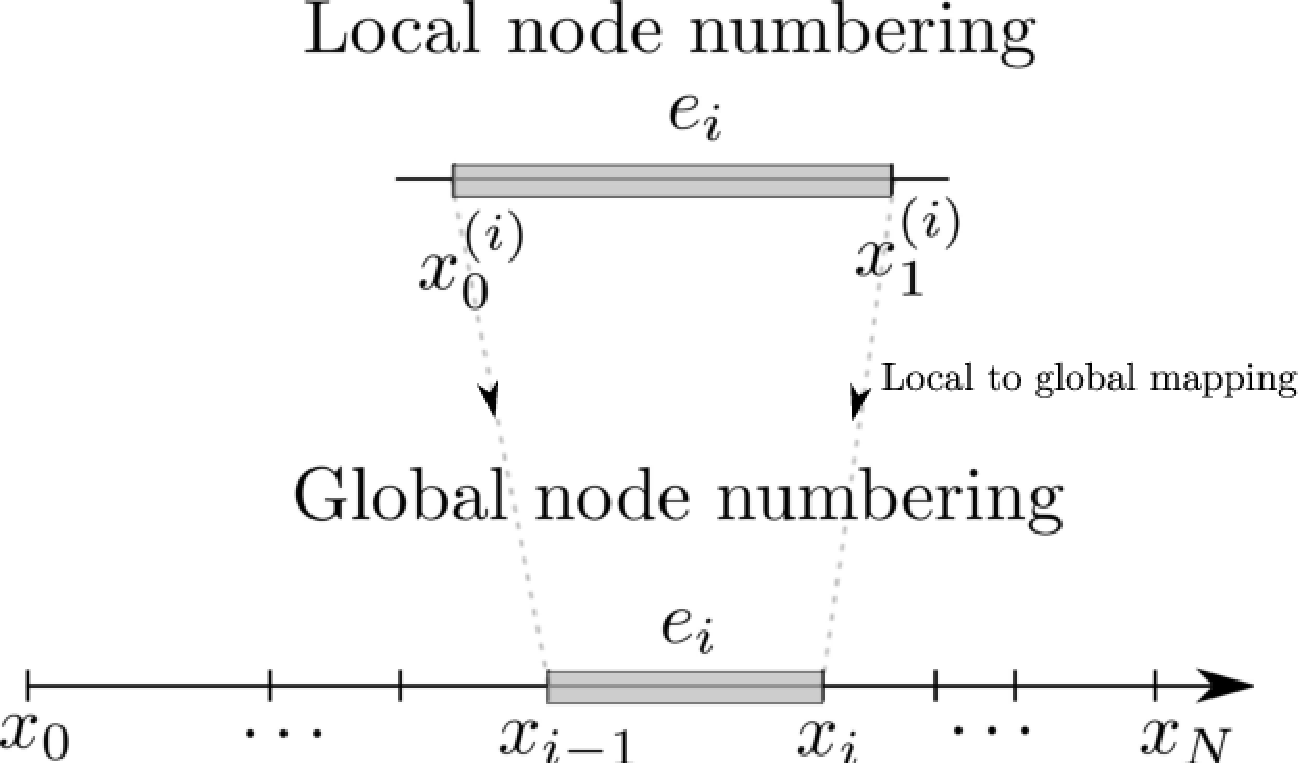
\includegraphics[width=0.8\textwidth]{./images/local_global_numbering}
  \caption{The local and global numbering schemes for nodes in a one-dimensional
    finite element model.}
  \label{fig:local-global-numbering}
\end{figure}

The process of assigning a global node number to each local node is known as the local to global mapping.
Good book keeping of the mapping is essential, especially in higher dimensions when this it becomes much more complex.

We define the local basis functions in element $e$ as
\begin{equation}
  L_{0}^{(e)}(x)=\dfrac{x-x_{1}^{(e)}}{x_{0}^{(e)}-x_{1}^{(e)}},\qquad
  L_{1}^{(e)}(x)=\dfrac{x-x_{0}^{(e)}}{x_{1}^{(e)}-x_{0}^{(e)}}
  \qquad\text{for }x\in e=[x_{0}^{(e)},x_{1}^{(e)}].
  \label{eq:32}
\end{equation}
Except for the test functions when $\ndi$ is a boundary node.
In this case we define $L_\ndi^{(e)} = 0$.
The $\ndi$th global basis function is then defined as:
\begin{equation}
  \label{eq:33}
  L_\ndi(x) =
  \begin{cases}
    L_\ndi^{(e)}(x) & \text{if node $\ndi$ is in element $e$,} \\
    0 & \text{otherwise.}
  \end{cases}
\end{equation}

\begin{figure}
  \center
  % ??ds numbering: change e_i to element e, e_{i+1} to e+1, x_i to x_\ndi, x^(i) to x^(e) L_i to L_\ndi
  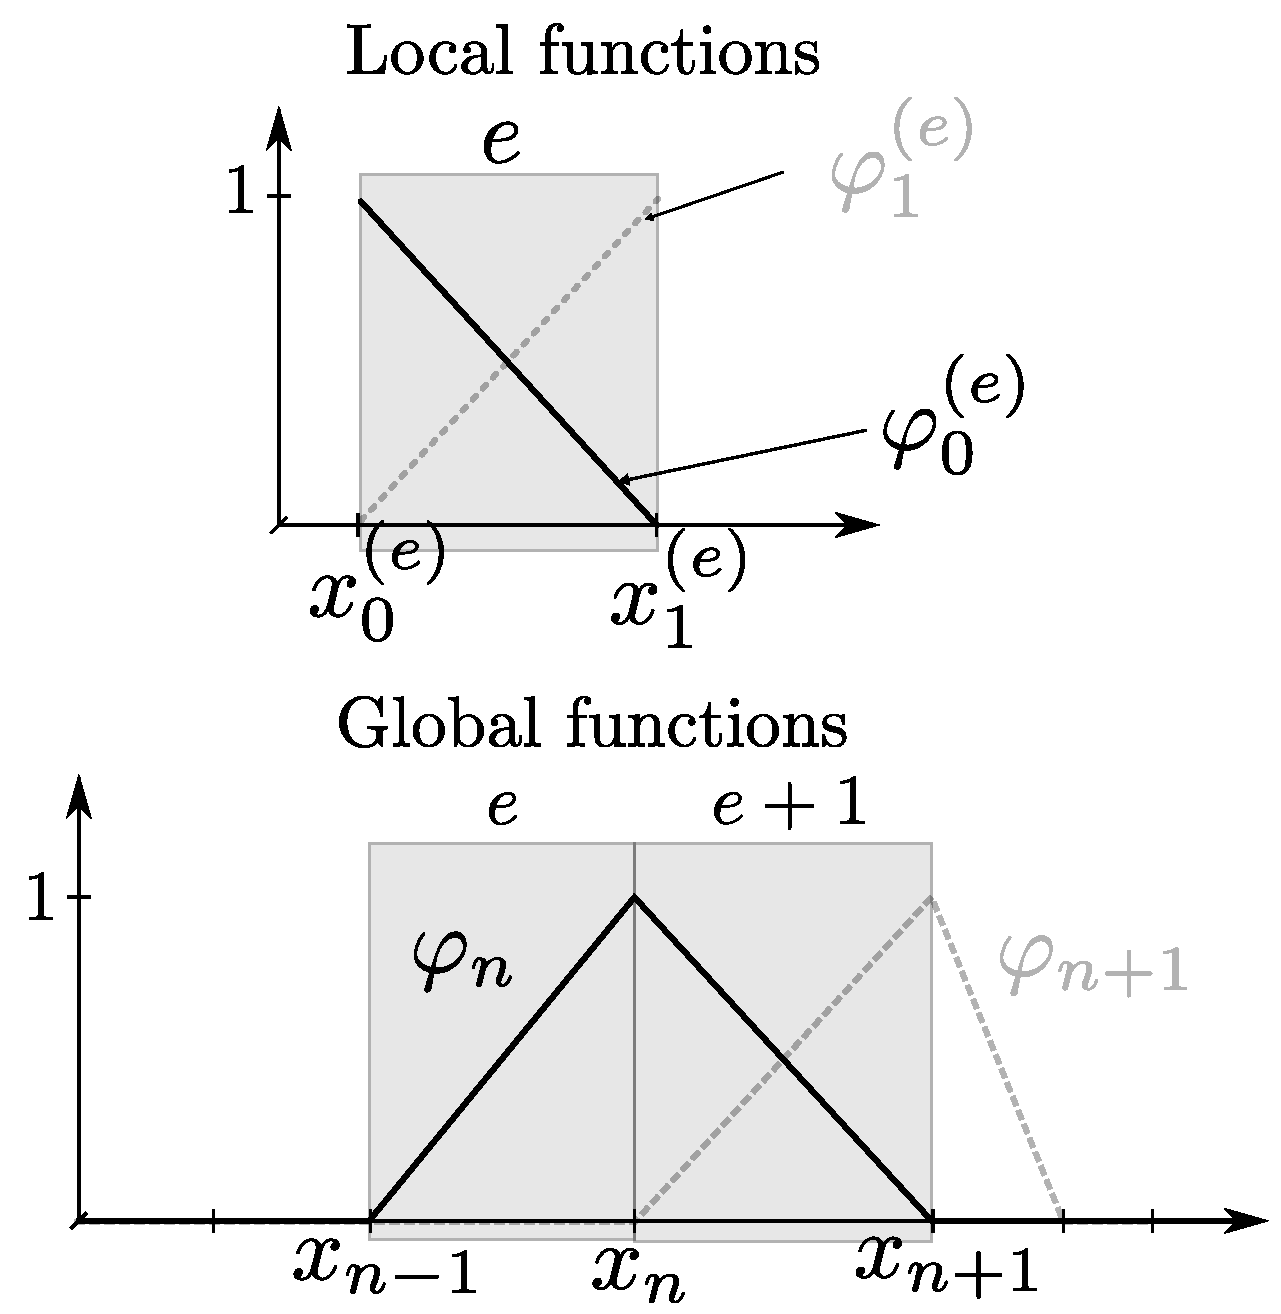
\includegraphics[width=0.8\textwidth]{./images/local_global_functions}
  \caption{The linear Lagrange basis functions and numbering schemes for a one-dimensional
    finite element model.\label{fig:local_global_functions}}
\end{figure}

The global basis functions for are clearly integrable (\ie in $L^2[0,1]$) since they are just a combination of local basis functions and they satisfy the boundary conditions by definition.
So the global basis functions are members of $V_T^h$ and $V_S^h$.

To calculate the matrix $A$ and the vector $\mathbf{b}$ from equation \eqref{eq:Aij_bj} needed for \eqref{eq:final_galerkin} we first calculate the local contributions from each element: $A^{(e)}$ and $\mathbf{b}^{(e)}$.
Then the local-to-global mapping tells us which local nodes map to a given global node and so the global $A$ and $\mathbf{b}$ can be assembled by summing the appropriate local contributions.

For our one-dimensional Poisson case the calculation of $A^{(e)}$ is quite
simple, substituting the two local basis functions \eqref{eq:32} into
\eqref{eq:Aij_bj} and using $h=x_{1}^{(e)}-x_{0}^{(e)}$ we are left with
\begin{equation}
  A^{(e)} = \dfrac{1}{h}
  \left[
    \begin{array}{cc}
      1 & -1 \\ -1 & 1
    \end{array}
  \right],
\end{equation}
where $h$ is the element size, $h = x_{1}^{(e)}-x_{0}^{(e)}$ (note that $h$ can vary between elements).
Similarly for $\mathbf{b}^{{e}}$ we obtain
\begin{equation}
  \mathbf{b}^{(e)}=\dfrac{1}{h}\left[
    \begin{array}{c}
      -\int_{x_{0}^{(e)}}^{x_{1}^{(e)}}(x-x_{1}^{(e)})\, f(x)\, dx\\
      \int_{x_{0}^{(e)}}^{x_{1}^{(e)}}(x-x_{0}^{(e)})\, f(x)\, dx
    \end{array}\right],
\end{equation}
which we compute numerically since the entries depend on $f(x)$ which is not yet decided.


% \subsection{Extension to other problems}

% \subsubsection{Non-Dirichlet Boundary Conditions}
% \label{sub:Non-Dirichlet-Boundary-Conditions}

% There are two main types of boundary condition.
% Dirichlet conditions specify the \emph{value} at the boundary (as used so far).
% Neumann conditions specify the \emph{derivative} at the boundary.
% These two types can also be mixed together either as conditions on different parts of the boundary or as a linear combination of the two (a Robin condition).

% Neumann boundary conditions can be added to the finite element method described above by relaxing the conditions on the shape and test functions at the boundary.
% Then the first term in equation~\eqref{eq:29} naturally gives an additional equation for the Neumann condition on each boundary node.

% Combinations of Neumann and Dirichlet conditions on different parts of the boundary can be treated the same way, by restricting the shape and test functions only on the Dirichlet parts.


% \subsubsection{Higher Order Shape/Test Functions}
% \label{sec:fem-high-order-shap}

% The shape and test functions can also be chosen to be of quadratic, cubic or higher order.
% This increases the number of nodes required per element (to ensure uniqueness) and increases the difficulty of calculating the integrals.
% However in some cases the use of higher order polynomials can give a better approximation.


% \subsubsection{Higher Dimensions}
% \label{sec:fem-higher-dimensions}

% The same basic method as given in \autoref{Derivation-of-weighted-residuals} and \autoref{sub:Actual-Finite-Elements} can be applied to two and three dimensional problems.
% Different polynomials for the shape/test functions must be chosen but the basic orthogonality property from equation~\eqref{eq:35} is kept.
% A larger variety of element shapes are possible -- typically triangular or quadrilateral elements are used in two dimensions and their higher dimension equivalents (tetrahedrons and ``bricks'') are used in three dimensions.


\subsection{Numerical evaluation of integrals}
% ??ds make sure I talk about quadrature in fem intro




\section{Initial Equations}
\label{sec:llg-initial-equations}

We start with the Gilbert form of the Landau-Lifshitz-Gilbert equation~\eqref{eq:Gilbert}, the sum of effective fields \eqref{eq:Heff}, the exchange field \eqref{eq:Hex} and the potential method for calculating the magnetostatic field \eqref{eq:Hms} \& \eqref{eq:nnphim}.

We use the Gilbert form of the Landau-Lifshitz-Gilbert equation even though it is less immediately intuitive because it greatly reduces the complexity of all derivatations--the Landau-Lifshitz form contains a double cross product term.
A side effect of this choice is that explict timestepping schemes cannot be used since the time dependence of the fundamental equation is defined implicitly.

After non-dimensionalisation (see \autoref{sec:land-lifsh-gilb-normalisation}) the Landau-Lifshitz-Gilbert equation with effective fields is given by
\begin{equation}
  \begin{aligned}
    \dmdt &= - \mv \times \hv + \alpha \mv \times \dmdt, \\
    \hv &= \happ - \nabla \phim + \lap \mv + \kone (\mv \cdot \ev) \ev, \\
    \lap \phim &= \div \mv.
    \label{eqn:ndllg-starting}
  \end{aligned}
\end{equation}

For now we consider the magnetostatic potential only within the magnetic domain, $\magd$, with Neumann or Dirichlet boundary conditions on the boundary, $\boundd$ (both cases will be required later, see \autoref{sec:hybr-finit-elem} for details of the extension to include the external region).
We define $\boundd_D$ and $\boundd_\Neu$ respectively to represent the region of the boundary domain where a Dirichlet condition or Neumann is imposed on the potential.
So $ \nabla \phim(\xv) \cdot \nv = g_\Neu(\xv) \; \forall \xv \in \boundd_\Neu$ and $\phim(\xv) = g_D(\xv) \; \forall \xv \in \boundd_D$.
Typically we will have either $\boundd_D = \boundd$ or $\boundd_\Neu = \boundd$.
We also define the following function spaces for convenience
\begin{align}
  \label{eq:037}
  \Dfs & = \set{ v \st v(\xv) \text{ satisfies the b.c. s } \; \forall \xv \in \boundd_D }, \\
  \Dfs_0 &= \set{ v \st v(\xv) = 0 \; \forall \xv \in \boundd_D }.
\end{align}

Recall from \autoref{sec:magn-bound-cond} that the boundary condition on the magnetisation is
\begin{equation}
  \label{eq:m-bc}
  \mv \times \dmdn = \zerov,
\end{equation}
It turns out that this Neumann-like condition is exactly what is needed in the derivation of the residuals.


\section{Conversion to Weak Form Residuals}

We convert some of the above equations into their residual weak forms as described in \autoref{Derivation-of-weighted-residuals}.
Each residual equation used increases the complexity of our system of equations, hence we do not rewrite the simple equations for crystalline anisotropy effective field or for the magnetostatic field (in terms of $\phim$) as residuals.


\subsection{Magnetostatic Field Residuals}
\label{sec:magn-field-resid}

The equation for the magnetostatic potential becomes \eqref{eq:phim} becomes:
\begin{gather}
  \text{given $\mv \in \sob^1(\magd)$, find $\phim \in \sob^2(\magd) \cap \Dfs$ such that:} \notag \\
  \rphi(\phim) = \int_\magd (\lap \phim) \test  \d \magd
  - \int_\magd (\nabla \cdot \mv) \test \d \magd = 0,
  \quad \forall \test \in \sob^0(\magd) \cap \Dfs_0. \label{eqn:phires1}
\end{gather}

The above equation for calculating $\phim$ contains second order derivatives.
We would like to reduce the order of these derivatives as discussed in \autoref{Derivation-of-weighted-residuals} to relieve the smoothness requirements on our solution.
We do this by ``transferring'' the derivatives onto the test functions \cite{HowardElmanDavidSilvester2006}.

First we need the following identity\footnote{This can be easily derived by applying the product rule to $\nabla \cdot (v \nabla \phim)$.}
\begin{equation}
  (\lap \phim) \test =
  \nabla \cdot (v \nabla \phim)
  - \nabla \phim \cdot \nabla v.
  \label{eq:20}
\end{equation}
Then integrating over the magnetic domain $\magd$ and applying the divergence theorem gives
\begin{equation}
  \int_\magd (\lap \phim) \test \d \magd =
  \int_{\boundd} \test (\nabla \phim \cdot \nv) \d \boundd
  - \int_\magd \nabla \phim \cdot \nabla \test \d \magd.
  \label{eqn:identitygauss}
\end{equation}

We now substitute \eqref{eqn:identitygauss} into \eqref{eqn:phires1}, giving
\begin{gather}
  \text{given $\mv \in \sob^1(\magd)$, find $\phim \in \sob^1(\magd) \cap \Dfs$ such that:} \notag \\
  \rphi(\phim) = \int_{\boundd} \test (\nabla \phim \cdot \nv) \d \boundd
  - \int_\magd \nabla \test \cdot \nabla \phim \d \magd
  - \int_\magd (\nabla \cdot \mv) \test \d \magd = 0
  , \notag \\
  \forall \test \in \sob^1(\magd) \cap \Dfs_0. \notag
\end{gather}
This contains only first order derivatives so the solution space for $\phim$ is relaxed to $\sob^1(\magd) \cap \Dfs$. However, all first partial derivatives of the test functions are now required to be integrable, \ie $v \in \sob^1(\magd)$ instead of $v \in \sob^0(\magd)$.

Note that the boundary integral is always zero on the Dirichlet region of the boundary by our definition of the test functions. Hence the boundary integral is only non-zero over $\boundd_{\Neu}$ where we know $(\nabla \phim \cdot \nv) = g_{\Neu}$. Hence we have
\begin{gather}
  \text{given $\mv \in \sob^1(\magd)$, find $\phim \in \sob^1(\magd) \cap \Dfs$ such that:} \notag \\
  \rphi(\phim) = \int_{\boundd_\Neu} \test g_\Neu \d \boundd
  - \int_\magd \nabla \test \cdot \nabla \phim \d \magd
  - \int_\magd (\nabla \cdot \mv) \test \d \magd = 0
  , \label{res:contphi} \\
  \forall \test \in \sob^1(\magd) \cap \Dfs_0. \notag
\end{gather}


\subsection{Landau-Lifshitz-Gilbert Equation Residuals}

For the Landau-Lifshitz-Gilbert equation~\eqref{eqn:ndllg-starting} we have a set of three residuals per test function. For now we sidestep the details of time discretisation by assuming $\dmdt$ to be just another function of $\xv$ that we can solve for.
\begin{gather}
  \text{given $\hv \in \sob^0(\magd)$ and $\mv \in \sob^1(\magd)$ find $\dmdt \in \sob^1(\magd)$ such that:} \notag
  \\
  \rllg(\mv) = \int_\magd \Big( \dmdt
  + (\mv \times \hca) + (\mv \times \happ) \\
  - (\mv \times \nabla \phi) + (\mv \times \lap \mv)
  - \dampc \left( \mv \times \dmdt \right)
  \Big) \cdot \testv \d\magd
  = 0, \label{res:contllg}
  \\
  \forall \testv \in (\sob^0(\magd))^3. \notag
\end{gather}

We again wish to reduce the order of the derivatives, this time on $\mv$ in
\begin{equation}
  I = \int_\magd (\mv \times \lap \mv) \cdot \testv \d\magd.
  \label{eq:46}
\end{equation}
First we reorder the terms to give
\begin{equation}
  \begin{aligned}
    I &= \intd{\lap \mv \cdot (\testv \times \mv)}, \\
      &= \intd{\lap \mv \cdot \bv}, \\
      &= \sum_{i=0}^2 \intd{\lap m_i \cdot b_i},
  \end{aligned}
\end{equation}
which is very similar to \eqref{??ds poisson}. So applying the same operations as used to obtain reduced derivatives in \autoref{Derivation-of-weighted-residuals} and \autoref{sec:magn-field-resid} we obtain
\begin{equation}
  I = \sum_{i=0}^2 \intb{b_i (\grad m_i \cdot \nv)} - \intd{\grad b_i \cdot \grad m_i}.
\end{equation}

It turns out that the first term is exactly the weak form of the boundary condition from \eqref{eq:m-bc}.
\begin{equation}
  \begin{aligned}
    \sum_{i=0}^2 \intb{b_i (\grad m_i \cdot \nv)} 
    &= \intb{\bv \cdot \pd{\mv}{\nv}}, \\
    &=  \intb{(\testv \times \mv) \cdot \pd{\mv}{\nv}}, \\
    &=  \intb{(\mv \times \pd{\mv}{\nv}) \cdot \testv}.
  \end{aligned}
\end{equation}
Hence for the case of no surface anisotropy this term is zero.

Next we need an expression for $\grad b_i$.
To avoid switching to tensor notation it is helpful to define $\grad \av = (\grad a_0, \grad a_1, \grad a_2)$.
Then using the product rule we have
\begin{equation}
  \begin{aligned}
    \grad \bv &= \grad \bigb{\testv \times \mv}, \\
    & = \grad \testv \times \mv + \testv \times \grad \mv.
  \end{aligned}
\end{equation}
Hence
\begin{equation}
  I = - \intd{\grad \mv : \bigb{\grad \testv \times \mv}} 
      - \intd{\grad \mv : \bigb{\testv \times \grad \mv}},
\end{equation}
where ``$:$'' is the componentwise scalar product $\grad \av : \grad \cv = \grad a_0 \cdot \grad b_0 + \grad a_1 \cdot \grad b_1 + \grad a_2 \cdot \grad b_2$.
The second term of this expression is zero by the properties of the triple product, so after reordering some terms we are left with
\begin{equation}
  \label{eq:final-lap-residual}
  I = - \intd{\bigb{\mv \times \grad \mv} : \grad \testv}.
\end{equation}


??ds write about switching to scalar test functions


\section{Spatial Discretisation}
\label{sec:spat-discr-resi}

The next step is to discretise the residuals in space. As in \autoref{Derivation-of-weighted-residuals} and \ref{sub:Actual-Finite-Elements} we replace continuous variables and functions by a basis representation using a finite space of shape functions. We also replace the infinite spaces of test functions used so far by finite dimensional approximations.

We choose the solution space to be the same as the test function space (except for boundary conditions), this choice makes our method a Galerkin method. We also choose the shape/test functions to be the same for all residuals/unknowns. So the infinite dimensional space used for all shape and test functions is $\sob^1(\magd)$ with appropriate boundary conditions.

We then replace the space $\sob^1(\magd)$ by the $N$-dimensional approximation $\ts \subset \sob^1(\magd)$. In this approximation the unknowns $\mv$, $\hex$ and $\phim$ can be represented anywhere in the domain as a sum over the nodal values multiplied by the shape function, $\sk \in \ts$, for that node:
\begin{gather} % \sk = shapefn_k
  \mv = \sum_{k = 0}^{N} \sk \, \mv_k, \quad
  \hex = \sum_{k = 0}^{N} \sk \, \hex_{,k}, \quad
  \phim = \sum_{k = 0}^{N} \sk \, \phim_{,k}.
  \label{eq:unknowns-basis}
\end{gather}
Similarly the test functions can be approximated by a sum over the test basis functions, $\tn \in \ts$, as
\begin{equation}
  \label{eq:47}
  \testv = \sum_{\ndi = 0}^{N} \tn \, a_\ndi.
\end{equation}
Note that in our method $\sbf_k \equiv \tbf_k$, but we continue to write the two functions differently for generality. Also the basis functions for the space of test functions are often simply refered to as the test functions since they are used equivalently.

So substituting the basis representations, \eqref{eq:unknowns-basis} and \eqref{eq:47} into the residuals we obtain a spatially discretised version of the problem.

% Note that we could move the discretised values of the unknowns outside of the integrals because they are constant in space. However we prefer to evaluate values at points within the elements where possible (by integrating using Gaussian quadrature) since some quantities are discontinous at the nodes.\footnote{For example if the basis functions are linear then derivatives are discontinous at the nodes.}

% Also note that we have $7N$ equations in $7N$ unknowns and each of the integrals in the equations can be evaluated only in terms of the shape/test functions, their derivatives, the outward unit normal vector and the Neumann boundary condition. Hence we have a system of algebraic equations which we can solve.

As described in \autoref{sub:Actual-Finite-Elements} we can convert this ``global'' representation into a number of ``local'' representations -- one on each element. We first split the domain into $N_e$ elements. We then define the basis functions such that they are only non-zero on elements in which they are contained (\ie we are using a finite element method). Then the global residuals can be split into the local contributions each element which are easy to calculate since they only depend on nodes within the element.\footnote{Unfortunately this property will be lost to some extent when we introduce the hybrid FEM/BEM in \autoref{sec:hybr-finit-elem}.}

Let $\magd_\eli$ represent the volume of element $e$, let $\boundd_\eli$ represent any part of the boundary of the element which is on $\boundd$ (nothing for most elements). Then the contribution of element $\eli$ to the residuals at node $\ndi$ is exactly as given in equations~\eqref{res:tintro}-\eqref{res:tllg} except that the integrations are performed over $\magd_\eli$ and $\boundd_\eli$ rather than $\magd$ and $\boundd$. Also note that the sums only need to consider values of $k$ such that node $k$ is in element $\eli$ and that residual contributions only need to be calculated for nodes $\ndi$ such that node $\ndi$ is in element $\eli$.


\section{Time Discretisation}
\label{sec:time-discretisation-resi}

To deal with the time derivative in the residual we apply a time discretisation scheme (\ie we use the method of lines). As discussed in \autoref{sec:model-conclusions} we aim to use the implicit midpoint rule in our final model but other methods are useful for comparison.

Let $\dtn$ be the time-step, let $\mv_k^\tl$ denote the value of $\mv_k$ at the $\tl$-th time-step, and consider only the value of $\mv_k$ at a single node. Then the mid-point method is defined by d'Aquino\cite{DAquino2005} as
\begin{equation}
  \label{eq:mid-point-scheme}
  \dmdt \left( \frac{\mv_k^{\tl+1} + \mv_k^\tl}{2} \right) = \frac{\mv_k^{\tl+1} - \mv_k^l}{ \dtn}.
\end{equation}
So by substituting equation~\eqref{eq:mid-point-scheme} into the spatially discretised residuals with $\mv_k = \frac{\mv_k^{\tl+1} + \mv^\tl_k}{2}$ we obtain a fully discretised system of equations in  $\mv_k^{\tl+1}$ and $\mv_k^\tl$.
Alternatively we can write it in terms of half a step of the first order backwards Euler method followed by a simple algebraic update \cite{Malidi2005}
\begin{equation}
  \label{eq:imr-bdf1}
  \begin{aligned}
    \dmdt \left(\mv_k^{l+\half} \right) &= \frac{\mv_k^{l+\half} - \mv_k^{l}}{\dtn/2}, \\
    \mv_k^{l+1} &= 2\mv_k^{l+\half} - \mv_k^l.
  \end{aligned}
\end{equation}


The constant time step second order backwards difference method is defined as\cite{Atkinson2009}
\begin{equation}
  \label{eq:bdf2-scheme}
  \dmdt(\mv_k^{\tl+1}) = \frac{3 \mv_k^{\tl+1} - 4 \mv_k^{\tl} + \mv_k^{\tl-1}}{2\dtn},
\end{equation}
which can similarly be substituted into the spatially discretised residuals with $\mv_k = \mv_k^{\tl+1}$ to obtain a fully discretised system of equations in of $\mv_k^{\tl+1}$, $\mv_k^\tl$ and $\mv_k^{\tl-1}$.


\section{Jacobian calculation}
\label{sec:llg-jacobian-calculation}

To solve this system by a Newton method we also need to know the Jacobian matrix of the residuals differentiated with respect to the variables at the target time step: $\phim_\ik^{\tl+1}$ and $\mv_\ik^{\tl+1}$.

\subsection{Poisson Jacobian}
\label{sec:poisson-jacobian}

Starting from the Poisson residual equation~\eqref{??ds poisson} and dropping terms that obviously contain no dependence on $\phim$ we get
\begin{equation}
  \begin{aligned}
    \label{eq:poisson-jacobian}
    \Am_{n,l} &= \pd{}{\phim_{,l}} \sum_k \intd{ -(\nabla \tbf_n \cdot \nabla \sbf_k) \phim_{,k}}, \\
    &= -\intd{\grad \tbf_n \cdot \grad \sbf_l}.
  \end{aligned}
\end{equation}
This block of the Jacobian is comparatively simple because the Poisson equation is linear. 
It corresponds to the well known discrete Laplacian operator\cite{HowardElmanDavidSilvester2006}.


\subsection{LLG Jacobian}
\label{sec:llg-jacobian}

We first note that the effect of differentiation on a single interpolated value is quite simple
\begin{equation}
  \pd{}{\mv_l} \left( \sum_k \mv_k \sk \right) = \sbf_l \text{I}_3.
\end{equation}
Unfortunately in most of the Jacobian calculations we have multiple terms depending on $\mv$ joined together by a cross product.
The process of differentiating these terms can be made much easier by making use of the ``skew operator'' which represents a cross product as a small matrix-vector multiplication.
The skew operator is given by
\begin{equation}
  \skewm{\av} = \text{skew}(\av) =
  \begin{pmatrix}
    0 & -a_3 & a_2 \\
    a_3 & 0 & -a_1 \\
    -a_2 & a_1 & 0
  \end{pmatrix}.
  \label{eqn:skew}
\end{equation}

Some properties are:
\begin{itemize}
\item Skew-matrix-vector multiplication is a cross product
  \begin{equation}
    \skewm{\av} \cdot \bv
    = \begin{pmatrix}
      0 & -a_3 & a_2 \\
      a_3 & 0 & -a_1 \\
      -a_2 & a_1 & 0
    \end{pmatrix}
    \cdot \threevec{b_1}{b_2}{b_3}
    = \threevec{-a_3b_2 + a_2b_3}{a_3b_1 - a_1b_3}{-a_2b_1 + a_1b_2}
    = \av \times \bv
  \end{equation}

\item No effect on derivatives
  \begin{equation}
    \pd{}{x} \skewm{\av} = \skewm{ \pd{\av}{x} }
  \end{equation}

\item Linearity
  \begin{equation}
    \skewm{\av + \alpha \bv} = \skewm{\av} + \alpha \skewm{\bv}
  \end{equation}

\item Easy to represent the Jacobian of a cross-product:

  \begin{equation}
    \pd{}{a_1} \skewm{\av} \cdot \bv = \begin{pmatrix}
      0 & 0 & 0 \\
      0 & 0 & -1 \\
      0 & 1 & 0
    \end{pmatrix}\bv = \threevec{0}{-b_3}{b_2}.
  \end{equation}
  Note that this is the first column of $-\skewm{\bv}$.
  It turns out that
  \begin{equation}
    \pd{}{\av} \skewm{\av} \cdot \bv = \begin{pmatrix}
      0 & b_3 & -b_2 \\
      -b_3 & 0 & b_1 \\
      b_2 & -b_1 & 0
    \end{pmatrix} = -\skewm{\bv}.
    \label{eq:61}
  \end{equation}

\item Simple behaviour when applied to interpolated values and differentiated:

  Due to linearity and the fact that all entries of $\pd{\mv_{l}}{\mv_{k}}$ are zero unless $l=k$ we have
  \begin{equation}
    \pd{}{\mv_l} \skewm{\intp{\mv}} \cdot \bv = \sum_k \sbf_k \pd{}{\mv_l} \bigb{\skewm{\mv_k} \bv} = \sbf_l \pd{}{\mv_l} \bigb{\skewm{\mv_l} \cdot \bv}.
  \end{equation}

  Then using \eqref{eq:61} we have
  \begin{equation}
    \pd{}{\mv_l} \skewm{\intp{\mv}} \cdot \bv = - \sbf_l\skewm{\bv}.
    \label{eq:diff-skew-interp}
  \end{equation}

\end{itemize}

Now note that combining the points above with the chain rule we get:
  \begin{equation}
    \begin{aligned}
      \pd{}{\mv_l} \bigb{\skewm{\mv}\cdot \gv(\mv)} 
      &= \skewm{\mv}\cdot \pd{\gv(\mv)}{\mv_l} - \sbf_l \skewm{\gv(\mv)}.
    \end{aligned}
  \end{equation}
In the context of the LLG Jacobian $\pd{\gv(\mv)}{\mv_l}$ is typically some scalar multiplied by an identity matrix.
Hence we can obtain a simple representation of most of the terms in the Jacobian in terms of the skew operator.

As a simple example of how this can be used we first examine the differentiation of the $\mv \times (\happ + \hms)$ term of the Landau-Lifshitz equation residual (note that these two fields are not (directly) dependant on $\mv$).
\begin{align}
  \circled{c} &= \intpb{\mv} \times (\happ + \hms), \notag\\
              &= \skewm{\intp{\mv}} \cdot (\happ + \hms).
\end{align}
Now it is easy to see that applying \eqref{eq:diff-skew-interp} gives us the Jacobian contribution
\begin{align}
  \pd{\circled{c}}{\mv_l} = - \sbf_l \skewm{\happ + \hms}.
\end{align}

Written using this skew operator the LLG residual is
\begin{equation}
  \begin{aligned}
    \rllg_n = \int_{\magd}
      & \dmdt \tbf_n \\
      &+ \skewm{\mv} \cdot \left( \happ + \hca - \nabla \phi - \dampc \dmdt
        \right) \tbf_n \\
      &- (\skewm{\mv} \grad \mv) : \grad \tbf_n)
      \d\magd
  \end{aligned}
\end{equation} 


Some more points before the main Jacobian calculation:
\begin{itemize}
\item Note that $\hca$ is a vector function of $\mv$ so differentiating it gives a 3x3 magnetocrystalline anisotropy Jacobian matrix $\Jmca$.

\item 
  \begin{equation}
    \begin{aligned}
      \pd{}{\mv_l} \left(\nabla \mv \compdot \nabla \tbf\right) 
      &= \pd{}{\mv_l} \threevecdup{\left( \sum_k \mv_k \grad \sbf_k \right) \cdot \grad \tbf}, \\
      &=  \sum_k \pd{\mv_k}{\mv_l} \threevecdup{\grad \sbf_k \cdot \grad \tbf}, \\
      &=  \Idm_3 \left(\nabla \sbf_l \cdot \nabla \tbf \right).
    \end{aligned}
  \end{equation}


\item We write
  \begin{equation}
    \Jmts \sbf_l = \pd{}{\mv_l} \left(\pd{\mv}{t} \right),
  \end{equation}
  where $\Jmts$ is some constant matrix that depends on the time integration scheme.
  For BDF2 $\Jmts = \frac{3}{2\dtn} \Idm_3$, for the implicit midpoint rule $\Jmts = \frac{1}{\dtn} \Idm_3$.
\end{itemize}


To simplify the calculations we write the Jacobian as the sum of simpler Jacobians:
\begin{equation}
  \begin{aligned}
    \Fm_{n,l} &= \pd{\rllg_n}{\mv_l} = A_{n,l} + B_{n,l} + C_{n,l}, \\
    A_{n,l} &= \pd{(\text{time residual})_n}{\mv_l}, \\
    B_{n,l} &= \pd{(\text{exchange residual})_n}{\mv_l}, \\
    C_{n,l} &= \pd{(\text{other residuals})_n}{\mv_l}.
  \end{aligned}
\end{equation}


First we calculate the simple Jacobian contribution due to the lone time derivative on the LHS
\begin{equation}
  \begin{aligned}
    A_{n,l} &= \pd{}{\mv_l} \intd{ \dmdt \tbf_n } \\
           &= \Jmts \intd{ \sbf_l \tbf_n}.
  \end{aligned}
\end{equation}
This is a 3x3 block diagonal matrix where each block is a simple mass matrix multiplied by the time integrator weight.

Next we calculate the contribution from damping and the various simple fields
\begin{equation}
  \begin{aligned} 
    C_{n,l} &= \pd{}{\mv_l} \intd{  \skewm{\mv} \cdot
      \left( \happ + \hca - \nabla \phi - \dampc \dmdt
      \right) \tbf_n}, \\
    &= \intd{ \tbf_n \sbf_l \left( -\skewm{\happ + \hca - \nabla \phi - \dampc \dmdt}
       + \dampc \jts \skewm{\mv}\right)}, \\
    &= \skewm{\intd{ \tbf_n  \sbf_l \left( \nabla \phi + \dampc \dmdt
          + \dampc \jts \mv - \happ - \hca \right) }}.
  \end{aligned}
\end{equation}
This is a 3x3 block skew-symmetric matrix where each block is something like a mass matrix multiplied by a collection of field/magnetisation components.

Finally we calculate the most complex term: the exchange contribution
\begin{equation}
  \begin{aligned}
    B_{n,l} &=  \pd{}{\mv_l} \intd{- \skewm{\mv} \cdot (\grad \mv \compdot \grad \tbf_n)} ,\\
    &= \intd{ \sbf_l \skewm{\grad \mv \compdot \grad \tbf_n}
       - \skewm{\mv} \left( \nabla \sbf_l \cdot \nabla \tbf \right)}, \\
     &= \skewm{ \intd{ \sbf_l \left( \grad \mv \compdot \grad \tbf_n \right)
         - \mv \left( \nabla \sbf_l \cdot \nabla \tbf \right)}}.
   \end{aligned}
 \end{equation}
We can simplify this slightly more by expanding the shape function representation and using chain rule
\begin{equation}
  \begin{aligned}
    B_{n,l} &= \skewm{ \sum_k \intd{ \sbf_l \left( \mv_k \grad \sbf_k \compdot \grad \tbf_n \right)
        - \mv_k \sbf_k \left( \nabla \sbf_l \cdot \nabla \tbf \right)}}, \\
    &= \skewm{ \sum_k \intd{ \bigb{(\sbf_l \grad \sbf_k - \sbf_k \grad \sbf_l)
        \cdot \grad \tbf_n}  \mv_k }}. \\
  \end{aligned}
\end{equation} 
So again we have a 3x3 block skew-symmetric matrix.
However this time each block is something like a Laplacian block (two derivatives).


When written in block form the total LLG Jacobian is
\begin{equation}
  \Fm =
  \begin{pmatrix}
    \jts \Mm    & -\Km_z       & \Km_y \\
    \Km_z         & \jts\Mm    & -\Km_x \\
    -\Km_y        & \Km_x        & \jts \Mm
  \end{pmatrix}, 
\end{equation}
where $\Mm$ is the mass matrix
\begin{equation}
  \label{eq:mass-matrix}
  \Mm_{i,j} = \intd{\tbf_i \sbf_j},
\end{equation}
and $\Km_i$ are the various contributions from $B$ and $C$.

\section{LLG-magnetostatics coupling Jacobians}
\label{sec:llg-magn-coupl}

Now we derive the Jacobian entries corresponding to $\Pm = \pd{\rllg}{\phim}$ and $\Qm = \pd{\rphi}{\mv}$.

First $\Pm$, obviously most of the terms in the llg residual are dropped when differentiated with respect to any $\phim_{,i}$ value so the calculation is quite simple
\begin{equation}
  \begin{aligned}
    \Pm_{n,l} &= \pd{\rllg_n}{\phim_l} 
    = \pd{}{\phim_l} \intd{ -\tbf_n \mv \times \grad \phim}, \\
    &= -\intd{ \tbf_n \mv \times \grad \sbf_l}, \\
    &= -\intd{ \tbf_n \threevec{m_y\pd{\sbf_l}{z} - m_z \pd{\sbf_l}{y}}
      {-m_x\pd{\sbf_l}{z} + m_z \pd{\sbf_l}{x}}
      {m_x\pd{\sbf_l}{y} - m_y \pd{\sbf_l}{x}}}.
  \end{aligned}
\end{equation}
Note that this is a $3 \times 1$ block matrix because we are dealing with a vector of three residuals at once.

Next $\Qm$, which will be a $1 \times 3$ block matrix because we are dealing with differentiation by three variables (the three components of $\mv$) at once.
\begin{equation}
  \begin{aligned}
    \Qm_{n,l} &= \pd{\rphi_n}{\mv_l} = \pd{}{\mv_l} \intd{ -\tbf_n \div \mv}, \\
    &= \pd{}{\mv_l} \intd{ \sum_j -\tbf_n \div (\sbf_j \mv_j)}, \\
    &= \pd{}{\mv_l} \intd{ \sum_j -\tbf_n \left( \pd{\sbf_j}{x} m_{x,j} 
        + \pd{\sbf_j}{y} m_{y,j} + \pd{\sbf_j}{z} m_{z,j} \right) }, \\
    &= -\intd{ \tbf_n \left( \pd{\sbf_l}{x}, 
        \pd{\sbf_l}{y}, \pd{\sbf_l}{z} \right) }, \\
    &= -\intd{\tbf_n (\grad \sbf_j)^T}.
  \end{aligned}
\end{equation}

So in block form the complete Jacobian is
\begin{equation}
  \Jm =
  \begin{pmatrix}
    \jts \Mm    & -\Km_z       & \Km_y      & \Pm_x \\
    \Km_z         & \jts\Mm    & -\Km_x     & \Pm_y \\
    -\Km_y        & \Km_x      & \jts \Mm & \Pm_z \\
    \Qm_x       & \Qm_y      & \Qm_z    & \Am     \\
  \end{pmatrix},
\end{equation}
where $\Am$ is the Poisson Jacobian.
Alternatively
\begin{equation}
\Jm =
  \begin{pmatrix}
    \Fm   & \Pm \\
    \Qm   & \Am \\
  \end{pmatrix}.
\end{equation}



\section{Geometric integration with the finite element method}
\label{sec:nodal-integration}

% ??ds add less than ntol to end of other residuals elsewhere?

In weak form methods such as FEM (see \autoref{sec:intr-finite-ele-diff}) it turns out that standard (\ie Gaussian) quadrature schemes do not retain the conservation properties of the IMR.
The problem is that (outside of the infinite node limit) weak form equations make statements about the integral properties of the solution, whereas magnetisation length is a nodal property.
The solution is to use an alternative quadrature scheme which directly links the nodal values with the integral values.
The downside of such a scheme is that the accuracy of the evaluation of integrals is reduced (since the standard schemes are chosen for their optimal accuracy).

In the micromagnetics literature this is known as reduced integration \cite{Cimrak2008}.
However in other finite element literature ``reduced integration'' refers to using a lower order Gaussian quadrature than needed to exactly integrate the shape and test functions.
The term ``Nodal integration'' is more the standard term for schemes where the nodal values are used directly in the quadrature (typically with mesh-free methods \eg \cite{Puso2008}).

In this section we first show why standard quadrature schemes cannot have the required conservation properties.
We then show that the introduction of nodal integration schemes reattains the conservation properties.
Finally we present some numerical experiments.


\subsection{Gaussian integration}

\subsubsection{Failure of $\abs{\mv}$ conservation with Gaussian quadrature}

\newcommand{\ipg}[2]{\intd{{#1} \cdot {#2}}}

We begin with the weak form of the LLG equation
\begin{equation}
  \label{eq:weak-llg}
  \intd{\dmdt \cdot \testv + \mv \times \hv[t, \mv] \cdot \testv - \dampc \mv \times \dmdt \cdot \testv} = 0, \quad \forall \testv
\end{equation}
where $\testv = \threevec{\test}{\test}{\test}$ and $\test \in \ts$ is a scalar test function.

\newcommand{\midpoint}[1]{\hat{#1}}
\newsubcommand{\mvm}{\midpoint{\mv}}{n}
\newcommand{\tm}{\midpoint{t}_n}

\newcommand{\pdsub}[3]{\mathrlap{\pd{#1\mathrlap{_{#2}}}{#3}}\phantom{\pd{#1_{#2}}{#3}}}
\newcommand{\dtop}{\delta}
\newcommand{\dmdtm}{\pdsub{\mv}{n}{t}}
\newcommand{\dmdtml}{\pdsub{\mv}{n,l}{t}}
\newcommand{\dmdtmj}{\pdsub{\mv}{n,j}{t}}

% To simplify the notation we use inner product notation for the integral of a dot product:
% \begin{equation}
%   \intd{\av \cdot \bv} = \ipg{\av}{\bv}.
% \end{equation}

Substituting in the IMR we obtain
\begin{equation}
  \label{eq:weak-llg-imr}
  \ipg{\dmdtm}{\testv} + \ipg{(\mvm \times \hv[\tm, \mvm])}{\testv} - \dampc \ipg{(\mvm \times \dmdtm)}{\testv} = 0, \quad \forall \testv .
\end{equation}

where $\midpoint{x} = \frac{x_{n+1} + x_{n}}{2}$ is the midpoint value of $x$ and $\dtop x = \frac{x_{n+1} - x_n}{\dtn}$ is the midpoint derivative.

To obtain our result we examine the case where $\testv = \mvm$.
Note that $\mvm$ is in the vector space of test functions because we are using identical test and shape function spaces and $\mvm$ at any point must only be a linear combination of shape functions.
So by \eqref{eq:weak-llg-imr}, and using the fact that $(\av \times \bv) \cdot \av) = 0$ we have
\begin{equation}
  \label{eq:23}
  \begin{aligned}
    0 &= \ipg{\dmdtm}{\mvm}, \\
    &= \frac{1}{2\dtn} \intd{(\mv_{n+1} + \mv_{n}) \cdot (\mv_{n+1} - \mv_n)}, \\
    &= \frac{1}{2\dtn} \intd{\abs{\mv_{n+1}}^2 - \abs{\mv_{n}}^2}.
  \end{aligned}
\end{equation}

At first glance it appears that we have achieved conservation. However this is only an integral relationship, meaning that the values of the integrand at the nodes are not constrained.
We can see this in more detail by substituting in the space interpolation of $\mv$ at the Gaussian integral evaluation points.
Dropping the constant factor of $2\dtn$ and assuming that $\abs{\mv_n} = 1$ everywhere this gives
\begin{equation}
  \begin{aligned} 
    1 &= \intd{\abs{\sum_k \mv_{n+1, k} \tbf_k(\xv)}^2}, \\
    &= \sum_l w_l \abs{\sum_k \mv_{n+1, k} \tbf_k(\xv_l)}^2.
  \end{aligned} 
\end{equation}

This can be satisfied without requiring that all $\abs{\mv_{n+1, k}} = 1$.
For example if we set the number of nodes to two (a 1D problem with linear shape functions) and assume magnetisation only along the $z$-axis then this condition becomes:
\begin{equation}
  \begin{aligned}
    1 &= \sum_l w_l \abs{\sum_k \mv_{n+1, k} \tbf_k(\xv_l)}^2, \\
    &= w_0 (m_0 a + m_1 b)(m_0 a + m_1 b) + w_1 (m_0 c + m_1 d)(m_0 c + m_1 d), \\
    &= m_0^2 (w_0 a^2 + w_1 c^2) + m_1^2 (w_0 b^2 + w_1 c^2) + m_0 m_1 (2w_0ab + 2w_1cd), \\
    &= m_0^2 \alpha + m_1^2 \beta + m_0 m_1 \gamma, \\
  \end{aligned}
\end{equation}
where $a,b,c,d$ are the values of shape functions at the integration points, $m_l = m_{z}$ at node l and $\alpha, \beta, \gamma$ are constants.
So given any $m_{z,0}$ we can solve the above expression to find an $m_{z,1}$ that satisfies the constraint.
Since $m_z$ all magnetisation is along the $z$-axis in this example we can vary magnetisation length arbitrarily while still satisfying the constraint.

A similar expression is obtained if nodal magnetistations are chosen for the test function used in \eqref{eq:23} instead of the magnetisation function, as in \autoref{sec:weak-cons-absmv}.

Finally it is interesting to note that if the magnetisation is constant in space at times $t_n$ and $t_{n+1}$ then the integral condition in \eqref{eq:23} \emph{is} sufficient to give conservation of the magnetisation length at nodes.


\subsubsection{Failure of energy conservation with Gaussian quadrature}

The proof of energy conservation does not fail directly.
However, non-constant magnetisation length means that the derivation of the boundary condition is no longer applicable (??ds check this, non-constant |m| should destroy Neumann condition therefore symmetry is gone).
Hence the effective field is no longer symmetrical and the proof of energy conservation no longer applies.

\subsection{A local nodal integration scheme}

In order to regain conservation properties in a weak-form-based method we introduce a nodal integration scheme based on that used by Bartels et. al.\cite{Bartels2006}:
\begin{equation}
  \label{eq:nodal-integration}
  \int f(\xv) \d \xv \approx \sum_{l\in \text{nodes}} \beta_l f(\xv_l),
\end{equation}
where $\beta_l$ is a weight.
This is simply the weighted sum of the value of the integrand at nodes.

As an additional benefit this greatly simplifies the calculations since no interpolation of the values to the integration points is needed.
For example with reduced integration (and using that $\tbf_k(\xv_l) = \delta_{kl}$) the residual contribution of the time derivative term of LLG of test function $k$ becomes
\begin{equation}
  \begin{aligned}
    \intd{\dmdt \cdot \tbfv_k} &= \frac{1}{\dtn} \intd{(\mv_{n+1}(\xv) + \mv_{n}(\xv)) \cdot \tbfv_k(\xv)}, \\
    & = \frac{1}{\dtn} \sum_{l\in \text{nodes}} \beta_l (\mv_{n+1, l} + \mv_{n, l}) \cdot \tbfv_k(\xv_l), \\
    & = \frac{1}{\dtn} \beta_k (\mv_{n+1, k} + \mv_{n, k}) \cdot \threevec{1}{1}{1}.
  \end{aligned}
\end{equation}

% \subsubsection{Derivation of weights for local integration}

We now need to derive a suitable $\beta_l$.
To do so we represent the quadrature scheme as an integral of an interpolating polynomial which matches the desired integration scheme, then we rearrange the equation to find the weights (see, \eg \cite[480]{Kincaid2002}).
In \texttt{oomph-lib} all integration is done in local co-ordinates (as discussed in \autoref{sec:fem-integration-??ds}), so we now calculate weights applicable in this case.

A suitable quadrature-interpolation-polynomial for our case is the shape/test function for the node.
So we have:
\begin{equation}
  \label{eq:nodal-quad-weights}
  \begin{aligned}
    \int_{\magd_e} f(\xv) \d \xv &= \int_{\magd_e} f(\sv) \pd{\sv}{\xv} \d \sv, \\
    &\approx \int_{\magd_e} \sum_l f(\sv_l) \tbf_l(\sv) J_l \d \sv, \\
    &\approx  \sum_l f(\sv_l) J_l \int_{\magd_e} \tbf_l(\sv)  \d \sv,
  \end{aligned} 
\end{equation}
where $J_l =  \evalatb{\pd{\sv}{\xv}}{\sv=\sv_l}$ is the Jacobian of the transformation from local to global coordinates evaluated at the $l$-th integration point.
Comparing \eqref{eq:nodal-integration} with \eqref{eq:nodal-quad-weights} we see that
\begin{equation}
  \beta_l =  J_l \int_{\magd_e} \tbf_l(\sv)  \d \sv.
\end{equation}
The equivalent weight for global integration is $\beta_l = \int_{\magd} \tbf_l(\xv) \d \xv$, as used by Bartels \etal\cite{Bartels2006}.

If $f(\sv)$ is a linear polynomial then our nodal quadrature scheme is exact.
However most terms in the LLG residual are higher order, due to them containing one or more interpolated terms (each a linear polynomial) mulitiplied by a test function (also a linear polynomial).
An exception is the exchange residual, \eg the $x$-component:
\begin{equation}
  \begin{aligned}
    \rex_{,x} = - \intd{ m_y \bigb{\grad \tbf \cdot \grad m_z}} + \intd{ m_z \bigb{\grad \tbf_n \cdot \grad m_y}},
  \end{aligned}
\end{equation}
which is linear because the gradient terms are constants ($m_i$ and $\tbf_n$ are linear polynomials so their derivatives are constant).
Hence the exchange term is integrated exactly.



\subsubsection{Conservation of $\abs{\mv}$ at nodes}
\label{sec:weak-cons-absmv}

??ds add weak exchange residual!

Starting from the IMR discretised weak form of the LLG \eqref{eq:weak-llg-imr}, after minimising the residual we have that
\begin{equation}
  \intd{\dmdtm \cdot \testv + (\mvm \times \hv[\tm, \mvm]) \cdot \testv - \dampc (\mvm \times \dmdtm) \cdot \testv } < \ntol, \quad \forall \testv .
\end{equation}

Next we examine the choice of the test function as the midpoint nodal value of $\mv$ at node j multiplied by the $j$th test basis function, $\testv = \mvm_{,j} \tbf_j$.
This choice is clearly in the vector space of test functions because it is simply a constant multiple of a basis function.
The result is
\begin{equation}
  \sum_l \beta_l \jstox_l \bigs{\dmdtml \cdot \mvm_{,j}\tbf_j(\xv_l) + (\mvm_{,l} \times \hv[\tm, \mvm_{,l}]) \cdot \mvm_{,j}\tbf_j(\xv_l) - \dampc (\mvm_{,l} \times \dmdtml) \cdot \mvm_{,j}\tbf_j(\xv_l)} < \ntol.
\end{equation}

Using $\tbf_k(\xv_l) = \delta_{kl}$ we can eliminate the summation
\begin{equation}
  \beta_j \jstox_j \bigs{\dmdtmj \cdot \mvm_{,j} + (\mvm_{,j} \times \hv[\tm, \mvm_{,j}]) \cdot \mvm_{,j} - \dampc (\mvm_{,j} \times \dmdtmj) \cdot \mvm_{,j}} < \ntol.
\end{equation}
By the properties of the triple product the procession and damping terms vanish. Then expanding the midpoint values gives us our conservation result:
\begin{equation}
  \begin{aligned}
    \frac{\beta_j \jstox_j}{2\dtn}(\mv_{n+1,j} - \mv_{n,j}) \cdot (\mv_{n+1, j} + \mv_{n, j}) &< \ntol, \\
    \abs{\mv_{n+1, j}}^2 - \abs{\mv_{n, j}}^2 &< \frac{2\dtn}{\beta_j \jstox_j}\ntol.
  \end{aligned}
\end{equation}

This can obviously be repeated for all nodes $j$, hence each nodal magnetisation length is conserved.


\subsubsection{Energy loss}

??ds add weak exchange residual!


Again we start from the IMR discretised weak form of the LLG \eqref{eq:weak-llg-imr} and proceed by choosing specific test functions.
In this case we first choose $\testv = \dmdtm$, which gives:
\begin{equation}
  \label{eq:test-dmdt}
  \begin{aligned}
    \intd{\dmdtm \cdot \dmdtm} - \intd{\dmdtm  \cdot (\mvm \times \hv[\tm, \mvm])} < \ntol.
  \end{aligned}
\end{equation}

Secondly we choose $\testv = \hv[\tm, \mvm]$ to obtain:
\begin{equation}
  \label{eq:test-h}
  \begin{aligned}
    &\intd{\dmdtm \cdot \hv[\tm, \mvm]} - \dampc \intd{\hv[\tm, \mvm] \cdot (\mvm \times \dmdtm)} < \ntol \\
    &= \intd{\dmdtm \cdot \hv[\tm, \mvm]} - \dampc \intd{\dmdtm \cdot (\hv[\tm, \mvm] \times \mvm)}, \\
    &= \intd{\dmdtm \cdot \hv[\tm, \mvm]} + \dampc \intd{\dmdtm \cdot (\mvm \times \hv[\tm, \mvm])}.
  \end{aligned}
\end{equation}

Combining equations~\eqref{eq:test-dmdt} and \eqref{eq:test-dmdt} results in
\begin{equation}
  0 = \intd{\dmdtm \cdot \hv[\tm, \mvm]} + \dampc \intd{\dmdtm \cdot \dmdtm},
\end{equation}
\ie
\begin{equation}
  \intd{\mv_{n+1} \cdot \hv[\tm, \mvm]} = \intd{\mv_n \cdot \hv[\tm, \mvm]} - \dtn \dampc \intd{\dmdtm \cdot \dmdtm}.
\end{equation}
With zero applied field $\hv[t, \mv] = \hv[\mv]$ is a symmetrical linear operator on $\mv$ with respect to the inner product $\intd{\av \cdot \bv}$ (see \autoref{sec:energy-field-relation}), using this property in a similar manner to \autoref{sec:prop-imr-llg} we obtain
\begin{equation}
  \frac{1}{2}\intd{\mv_{n+1} \cdot \hv[\mv_{n+1}]} = \frac{1}{2}\intd{\mv_n \cdot \hv[\mv_n]} - \dtn \dampc \intd{\dmdtm \cdot \dmdtm}.
\end{equation}
But, as mentioned in \autoref{sec:prop-imr-llg} $\frac{1}{2}\intd{\mv \cdot \hv[\mv]}$ is the total micromagnetic energy of the domain (when $\happ = \zerov$), hence we have
\begin{equation}
  \e_{n+1} = \e_n - \dtn \dampc \intd{\dmdtm \cdot \dmdtm},
\end{equation}
which is the midpoint discretisation of the analytical energy loss rate given by equation~\eqref{eq:energy-decay}.
In particular when $\dampc = 0$ the energy is conserved.

The extension to the case with the applied field proceeds exactly as for the strong form of the LLG, as discussed in \autoref{sec:prop-imr-llg}.
The final result is
\begin{equation}
  ??ds
\end{equation}


\subsection{Numerical experiments}
\label{sec:numer-exper}

In the following experiments we use the wave exact solution in 2D (see \autoref{sec:wave-like-solution}) for simplicity and because an exact solution is known.
The solution parameters used are $\kvec = 2\pi$ so that the solution is periodic on domains of unit size and $c = 0.35\pi$ which gives large amplitude oscillations without while still remaining in the wave-like parameter regime.

The Newton tolerance is set to $10^{-14}$ unless otherwise specified.
The linear systems are solved using GMRES with an ILU-1 preconditioner.


\subsubsection{Accuracy of nodal quadrature}



\subsubsection{Convergence}

Since we have an exact solution for this example we can calculate the total error and plot the convergence as $\dtn \goesto 0$ and $h \goesto 0$.
Following the example of Jeong \etal\cite{Jeong2014} we link the spatial discretisation length to the time step by $\dtn = 0.32h$.

We plot two figures: convergence of a single step and convergence after some time.

??ds


\subsubsection{Magnetisation length conservation}

First we examine the evolution of the magnetisation length error over time in a single case.
We used $\dampc = 0.001$, a mesh of square elements with $6561$ nodes and constant time step sizes of $\dtn = 0.001$. 
These choices of mesh and time step resolve the solution well, as can be seen in the convergence experiments above.
The maximum time was $t_{max} = 5$ ($\approx 20$ wave periods), the damping is small enough that the oscillations continue well past this time. % trace in folder ??ds check it
\autoref{fig:mean-ml-error-2d-gauss} shows the behaviour of the maximum (over all nodes) error in magnetisation length, \autoref{fig:mean-ml-error-2d-nodal} shows the equivalent plot when using nodal quadrature.
When using nodal quadrature the error never grows much larger than the Newton tolerance, whereas when using Gaussian quadrature the error grows to $\order{10^{-5}}$ within the short simultation.

\begin{figure}
  \centering
  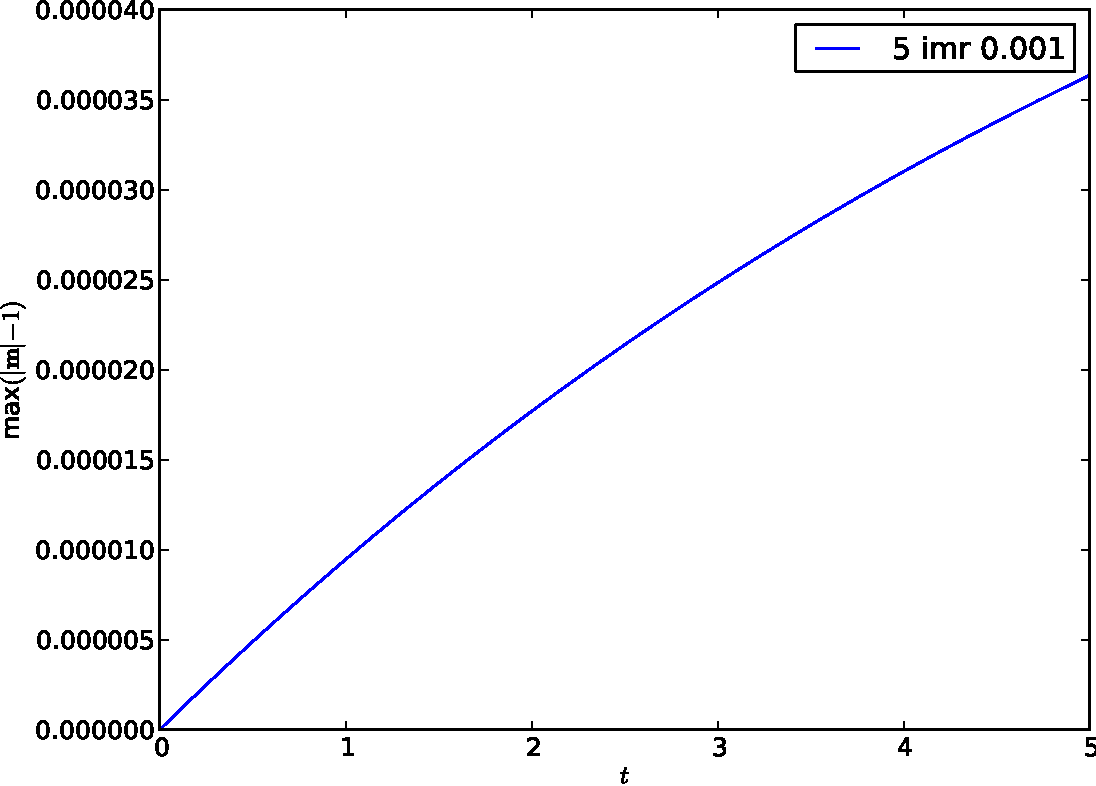
\includegraphics[width=0.8\textwidth]{plots/2d_wave_solution_m_length/gauss-maxmathbfm-1vst.pdf}
  \caption{Evolution of the maximum error of nodal magnetisation lengths in the 2D wave example with a standard Gaussian quadrature scheme.}
  \label{fig:mean-ml-error-2d-gauss}
\end{figure}

\begin{figure}
  \centering
  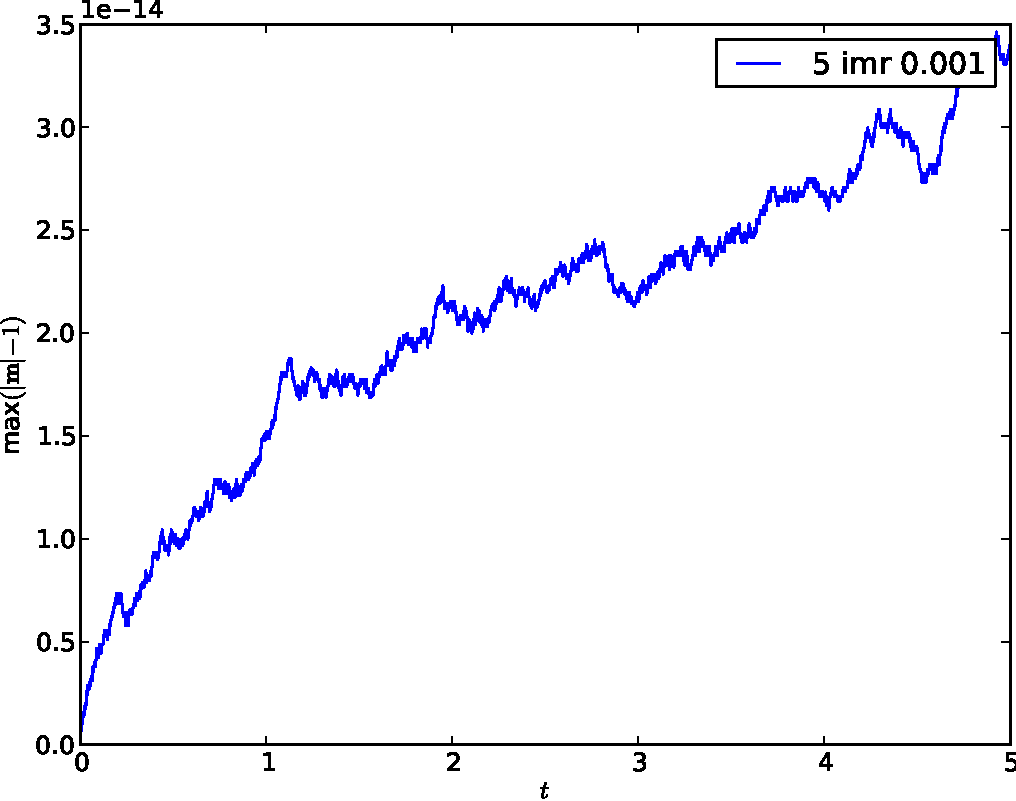
\includegraphics[width=0.8\textwidth]{plots/2d_wave_solution_m_length/lnodal-maxmathbfm-1vst.pdf}
  \caption{Evolution of the maximum error of nodal magnetisation lengths in the 2D wave example with the nodal quadrature scheme introduced above.}
  \label{fig:mean-ml-error-2d-nodal}
\end{figure}

To check that the conservation is independent of problem parameters we ran a parameter sweep using: square and triangle elements; 36, 441 and 6561 nodes; time steps of $0.1$, $0.01$ and $0.001$; and damping parameters of $1$, $0.1$, $0.001$ and $0$.
The maximum length error over all parameter sets, all time steps and all nodes when using nodal quadrature was 2.364775e-12, when using Gaussian quadrature it was 0.013746647.
This clearly demonstrates the necessity and effectiveness of the nodal quadrature scheme for retaining the conservation properties of the implicit midpoint rule.
% using the same data as for the figures above, look in their folders for parameter sets data parsing command: parse.py -d /mnt/moredata/optoomph/user_drivers/micromagnetics/experiments/parameter_sweeps/parameter_file_0/ -l=-dt -l=-damping --split=-integration --print-data max-max-ml --print-data ml -l=initial_nnode


??ds describe very long time behaviour in \autoref{fig:mean-ml-error-2d-nodal-long-time}.

\begin{figure}
  \centering
  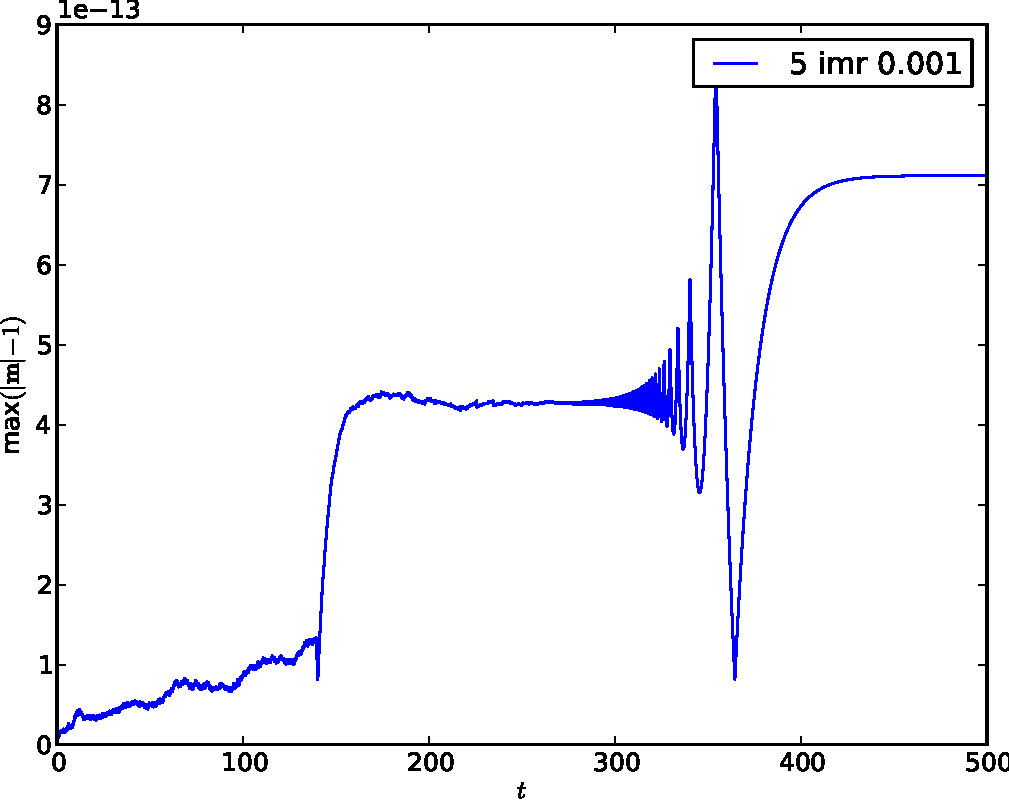
\includegraphics[width=0.8\textwidth]{plots/2d_wave_solution_m_length_long_time/-maxmathbfm-1vst.pdf}
  \caption{Evolution of the maximum error of nodal magnetisation lengths in the 2D wave example with the nodal quadrature scheme over a very long time period.}
  \label{fig:mean-ml-error-2d-nodal-long-time}
\end{figure}



\subsubsection{Effect of Newton tolerance}
\label{sec:effect-newt-toler-m-conservation}

Since the non-linear residual \eqref{eq:weak-llg} used in the derivation of the conservation properties is only true up to the accuracy of the linearisation method we would expect to see some effect when modifying this accuracy.
In our model Newton's method is used for linearisation (see \autoref{sec:newt-meth}) so the relevant measure of accuracy is the Newton tolerance.

The obvious experiment to carry out would be to vary the Newton tolerance and examine how the error in $\abs{\mv}$ is affected.
However Newton's method extremely quickly meaning that the final residual is sometimes orders of magnitude smaller than the tolerance, this would hide any corrolation between the tolerance and the error.
Instead we plot the error against the actual maximum residual obtained (specifically: the mean over time steps of $\norm{\rv}_\infty$ after the Newton method has converged). 
The results are shown in \autoref{fig:mean-ml-error-2d-nodal-newton-tests}, there is a clear corrolation between small residuals and small length errors.


\begin{figure}
  \centering
  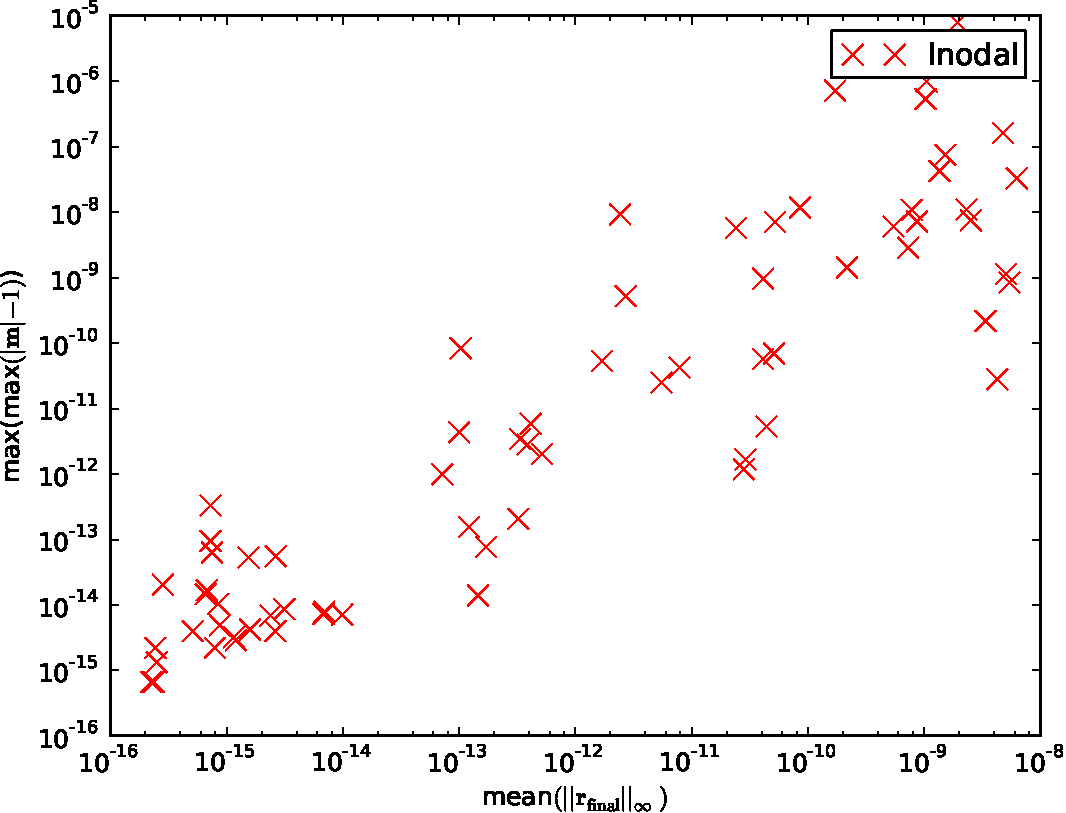
\includegraphics[width=0.8\textwidth]
  {plots/2d_wave_solution_m_length_newton_res/-maxmaxmathbfm-1vsmeanmathbfr_mathrmfinal_infty.pdf}
  \caption{Corrolation between maximum error of nodal magnetisation lengths and largest maximum Newton residual after convergence in the 2D wave example with the nodal quadrature scheme over a very long time period.}
  \label{fig:mean-ml-error-2d-nodal-newton-tests}
\end{figure}


\subsubsection{Adaptivity}
??ds - no need for this? leave it to the final subsection?

It remains to demonstrate that the adaptivity scheme introduced in \autoref{sec:adaptive-imr} is effective for the finite element problem with nodal integration.
Since there is still no relationship with previous time step sizes in the conservation proofs with nodal integration we don't expect there to be any issues with variable step size and conservation.

Additionally our discretisation can be written as semi-discretisation in space (giving a system of ODEs) followed by the application of IMR in time.
Hence we have no reason to expect the adaptive IMR to behave any differently to in the pure ODE case.

\subsubsection{BEM}
??ds - no need for this? leave it to the final subsection?


??ds


\subsection{Conclusions}

??ds


%%% Local Variables:
%%% mode: latex
%%% TeX-master: "main"
%%% End:
